\subsubsection{WPA2}

In 2004, the \gls{ieee} 802.11i amendment was finalized and published and, as planned, the \gls{wifi} Alliance released a new protocol based on the document, \gls{wpa}2 \cite{wifi_state}. Unlike its predecessor, \gls{wpa}2 wasn’t designed to work with older hardware constraints and could provide more robust security mechanisms.

One of the key differences between \gls{wpa} and \gls{wpa}2 is its confidentiality and integrity protocol. On \gls{wpa} it was optional to have the new protocol implemented, while on \gls{wpa}2 its implementation is mandatory and \gls{tkip} should only be used as a fallback for interoperability with older devices.

\gls{wpa}2 relies on the same authenticators of \gls{wpa}, \gls{psk} for \gls{wpa}2-Personal and \gls{ieee} 802.1X for \gls{wpa}2-Enterprise.

\paragraph{CCMP}

The \gls{ccmp} uses the \gls{aes} block cipher operating in \gls{ccm} mode. \gls{ctr} provides data confidentiality, while \gls{cbc}-\gls{mac} is used for authentication and integrity. Originally, \gls{ccmp} supported only 128-bit \gls{aes} keys (\gls{ccmp}-128), but later revisions of the algorithm allowed the use of 256-bit keys (\gls{ccmp}-256) as well.

\begin{figure}[h]
    \centering
    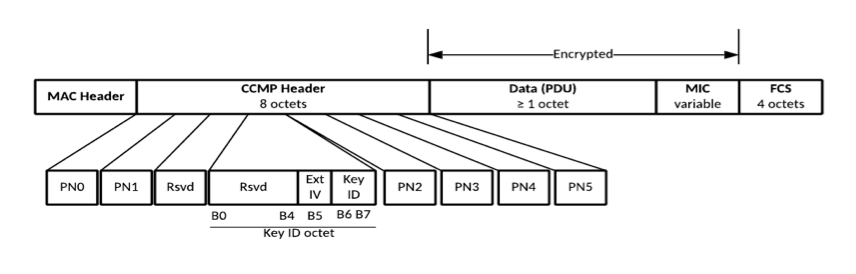
\includegraphics[width=\linewidth]{contents/background-in-wireless-networks/protected-network-standards/wpa2/ccmp/expanded-ccmp-mpdu.png}
    \caption{Expanded \gls{ccmp} \gls{mpdu}}
    {Source: \cite{ieee_80211_2020}}
    \label{figure:ieee80211_figure43n}
\end{figure}

Not needing to rely on \gls{wep} anymore, \gls{ccmp} unified the \gls{iv} field of \gls{wep} and \gls{eiv} field of \gls{wpa} into the 8-octet \gls{ccmp} Header field. The \gls{wep} \gls{icv} was dropped and the \gls{mic} field was turned into a variable size field, 8-octet or 16-octet long for \gls{ccmp}-128 and \gls{ccmp}-256 respectively. The resulting \gls{mpdu} is shown on Figure \ref{figure:ieee80211_figure43n}.

\begin{figure}[h]
    \centering
    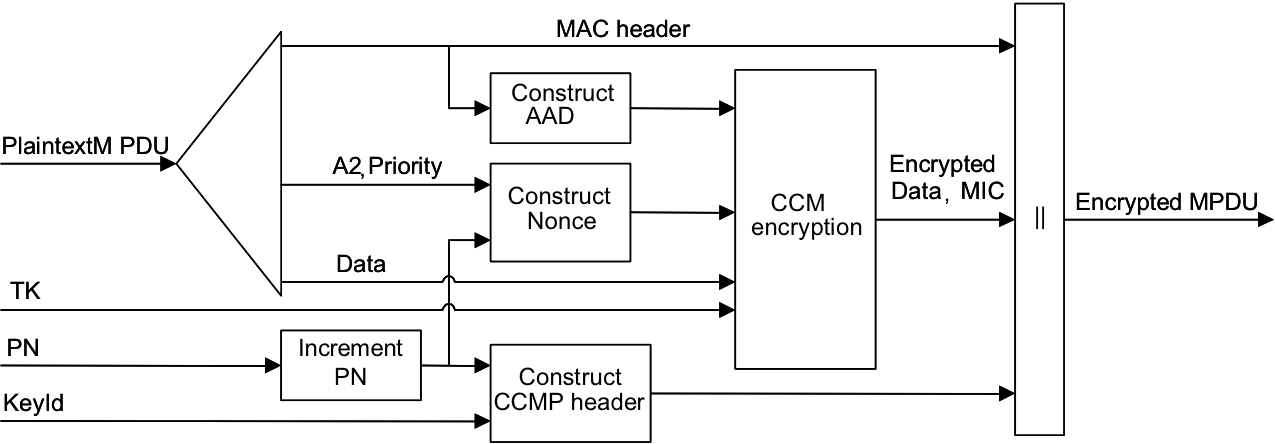
\includegraphics[width=\linewidth]{contents/background-in-wireless-networks/protected-network-standards/wpa2/ccmp/ccmp-encapsulation-block-diagram.png}
    \caption{\gls{ccmp} Encapsulation Block Diagram}
    {Source: \cite{ieee_80211_2020}}
    \label{figure:ieee80211_figure43o}
\end{figure}

On the encryption process, represented on Figure \ref{figure:ieee80211_figure43o}, \gls{ccmp} maintains a \gls{pn} value for each \gls{tk}, incrementing it sequentially for each \gls{mpdu} processed. The \gls{pn} is used along the \gls{kid} to build the \gls{ccmp} Header, part of the final \gls{mpdu}. \gls{pn} is also used together with the \gls{a2} and Priority of the \gls{mpdu} being consumed to calculate the Nonce Block, avoiding replay attacks. The \gls{mac} Header has its values authenticated by constructing the \gls{aad}, providing integrity protection. Finally, the \gls{ccm} Originator Processing is invoked with the values of \gls{aad}, nonce, plaintext, and \gls{tk} to form the ciphertext and the \gls{mic}. The encrypted \gls{mpdu} is accordingly assembled and sequentially transmitted.

\begin{figure}[h]
    \centering
    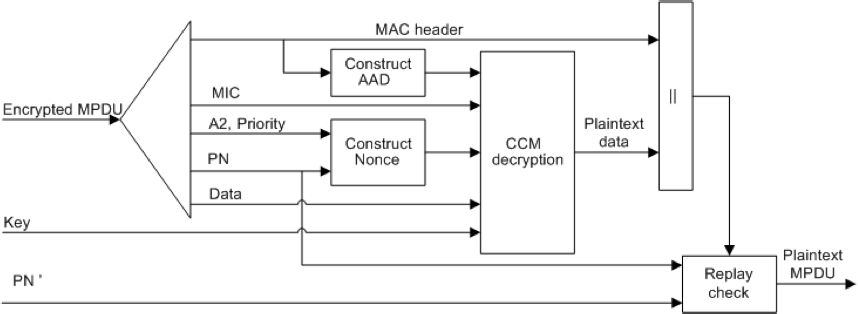
\includegraphics[width=\linewidth]{contents/background-in-wireless-networks/protected-network-standards/wpa2/ccmp/ccmp-decapsulation-block-diagram.png}
    \caption{\gls{ccmp} Decapsulation Block Diagram}
    {Source: \cite{ieee_80211_2020}}
    \label{figure:ieee80211_figure43r}
\end{figure}

To decrypt the \gls{mpdu}, the \gls{aad} is constructed in the same way as the original \gls{mpdu}. The Nonce Block uses the \gls{a2} and Priority values from \gls{mpdu} as usual, but it also gets the \gls{pn} from there. Then the \gls{ccm} Recipient Processing is invoked with the \gls{tk}, the calculated \gls{aad} and Nonce Block, and the extracted ciphertext and \gls{mic} values. The decrypted \gls{mpdu} is assembled with the resulting plaintext. Before having the \gls{mpdu} returned, the replay check is executed, which verifies if the extracted \gls{pn} value is less than or equal to the local \gls{pn} value for the \gls{tk}, implying a frame replay. The decryption process is shown on Figure \ref{figure:ieee80211_figure43r}.

\FloatBarrier

\paragraph{Security}

A compromise was made on the \gls{tkip} design to make possible its use on legacy \gls{wep} hardware. The forgery attacks were mitigated with the introduction of the Michael algorithm, but, due to computing power constraints, while blocking the forged packets it would cause a denial of service on the network \cite{ieee_80211_2020}.

As \gls{tkip} just encapsulates the \gls{wep} algorithm, it still relies on the security of the \gls{rc4} \gls{prng}. It was found that the keystream generated by \gls{rc4} is biased towards certain sequences and it made practical attacks against \gls{wpa}-\gls{tkip} networks within an hour \cite{rc4nomore}. The attacker would establish a \gls{tcp} connection with some victim on the network and would repeatedly send identical packets particularly sized with a well-known content over the connection. Then the wireless traffic was captured and filtered to only what would likely be an attacker's packet. Ciphertext statistics were extracted and plaintext likelihoods calculated using a combination of the \gls{fm} and \gls{absab} biases. Finally, the \gls{mic} key is derived from one of the candidates with the correct \gls{icv}, allowing any other packet of the victim to be fully decrypted.

